\documentclass[letterpaper,11pt,twoside]{article}
\usepackage[utf8]{inputenc}
\usepackage{amsmath,amsfonts,amssymb,amsthm,latexsym}
\usepackage[spanish,es-noshorthands]{babel}
\usepackage[T1]{fontenc}
\usepackage{lmodern}
\usepackage{graphicx,hyperref}
\usepackage{tikz,pgf}
\usepackage{multicol}
\usepackage{fancyhdr}
\usepackage[height=9.5in,width=7in]{geometry}
\usepackage{fancyhdr}
\pagestyle{fancy}
\fancyhead[LE]{
\includegraphics[height=12pt]{Images/logo-colegio.png} Álgebra $8^{\circ}$}
\fancyhead[RE]{}
\fancyhead[RO]{\textit{Germ\'an Avenda\~no Ram\'irez, Lic. U.D., M.Sc. U.N.}}
\fancyhead[LO]{}

\author{Germ\'an Avenda\~no Ram\'irez, Lic. U.D., M.Sc. U.N.}
\title{\begin{minipage}{.2\textwidth}

\includegraphics[height=1.75cm]{Images/logo-colegio.png}\end{minipage}
\begin{minipage}{.55\textwidth}
\begin{center}
Recomendaciones iii período, Polinomios\\
Álgebra $8^{\circ}$
\end{center}
\end{minipage}\hfill
\begin{minipage}{.2\textwidth}

\includegraphics[height=1.75cm]{Images/logo-sed.png} 
\end{minipage}}
\date{}
\thispagestyle{plain}
\begin{document}
\maketitle
Nombre: \hrulefill Curso: \underline{\hspace*{44pt}} Fecha: \underline{\hspace*{2.5cm}}\\

\fbox{\begin{minipage}{.99\textwidth}
Este trabajo debe ser realizado y entregado en las fechas que el colegio estipule, para luego ser sustentado.
\end{minipage}}

\begin{multicols}{2}
\section*{Adici\'{o}n y sustracci\'{o}n de polinomios}
 \subsection*{Conceptos}
 Para los items siguientes, responda V o F según el caso
 \begin{enumerate}
 \item El grado del monomio $4x^{2}y$ es 3
 \item Un polinomio de tres términos se denomina binomio
 \item Los términos de un monomio deben tener exponentes enteros por cada variable
 \item Si $3x-4$ es restado de $-7x+2$ su resultado es $8x-4$
 \item Si $-x-1$ es restado de la suma de $2x-1$ y $-4x-6$, se obtiene $-x-6$
 \end{enumerate}
 \subsection*{Problemas}
 Para los problemas siguientes, determine el grado del polinomio dado
 \begin{enumerate}
 \item $7xy+6y$
 \item $-x^{2}y+2xy^{2}-xy$
 \item $5x^{2}-7x-2$
 \item $8x^{6}+9$
 
Sume los polinomios

\item $3x-7$ \hspace*{.5cm} y \hspace*{.5cm} $7x+4$
\item $-5t-4$ \hspace*{.5cm} y \hspace*{.5cm} $-6t+9$
\item $3x^{2}-5x-1$ \hspace*{.5cm} y \hspace*{.5cm} $-4x^{2}+7x-1$
\item $12a^{2}b^{2}-9ab$ \hspace*{.5cm} y \hspace*{.5cm} $5a^{2}b^{2}+4ab$
\item $2x-4$,\hspace*{.5cm} $-7x+2$ \hspace*{.5cm} y \hspace*{.5cm} $-4x+9$

Reste los polinomios de los polinomios dados usando la forma horizontal

\item $5x-2$ de $3x+4$
\item $-4a-5$ de $6a+2$
\item $3x^{2}-x+2$ de $7x^{2}+9x+8$
\item $2a^{2}-6a-4$ de $-4a^{2}+6a+10$
\item $2x^{3}+x^{2}-7x-2$ de $5x^{3}+2x^{2}+6x-13$

Reste los polinomios usando la forma vertical

\item $5x-2$ de $12x+6$
\item $-4x+7$ de $-7x-9$
\item $2x^{2}+x+6$ de $4x^{2}-x-2$
\item $x^{3}+x^{2}-x-1$ de $-2x^{3}+6x^{2}-3x+8$
\item $-5x^{2}+6x-12$ de $2x-1$

Realice las operaciones descritas

\item Reste $2x^{2}-7x-1$ de la suma de $x^{2}+9x-4$ y $-5x^{2}-7x+10$
\item Reste $-x^{2}-7x-1$ de la suma de $4x^{2}+3$ y $-7x^{2}+2x$
\item Reste la suma de $5n^{2}-3n-2$ y $-7n^{2}+n+2$ de $-12n^{2}-n+9$

Realice las operaciones indicadas

\item $(5x+2)+(7x-1)+(-4x-3)$
\item $(12x-9)-(-3x+4)-(7x+1)$
\item $2x^{2}-7x-1)+(-4x^{2}-x+6)+(-7x^{2}-4x-1)$
\item $(7x^{2}-x-4)-(9x^{2}-10x+8)+(12x^{2}+4x-6)$
\item $(n^{2}-7n-9)-(-3n+4)-(2n^{2}-9)$

Simplifique quitando los paréntesis internos primero y luego los externos.

\item $3x-[5x-(x+6)]$
\item $2x^{2}-[-3x^{2}-(x^{2}-4)]$
\item $-2n^{2}-[n^{2}-(-4n^{2}+n+6)]$
\item $[4t^{2}-(2t+1)]-[3t^{2}+(2t-1)-5]$
\item $[2n^{2}-(2n^{2}-n+5)]+[3n^{2}+(n^{2}-2n-7)]$
\item $[7xy-(2x-3xy+7)]-(3x-(x-10xy-y)]$
\item $[4x^{3}-(2x^{2}-x-1)]-[5x^{3}-(x^{2}+2x-1)]$

Use geometría para resolver:

\item Encuentre el polinomio que representa el per\'{i}metro de cada figura
\begin{enumerate}
\item 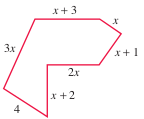
\includegraphics[scale=1]{Images/perimetro01.png}
\item 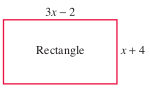
\includegraphics[scale=1]{Images/perimetro02.png} 
\end{enumerate}
\item Encuentre el polinomio que representa el área superficial del solido rectangular de la figura
\begin{center}
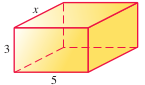
\includegraphics[scale=1]{Images/solido01.png} 
\end{center}
Ahora use el polinomio obtenido para determinar la superficie de los sólidos cuyas dimensiones se especifican:
\begin{enumerate}
\item 3 por 5 por 4
\item 3 por 5 por 13
\end{enumerate}
\item Encuentre el polinomio que representa el área superficial del cilindro circular recto de la figura. Después, use el polinomio obtenido para determinar él área superficial de los cilindros que tienen una base circular de radio 4. Puede usar la aproximación 3.14 para $\pi$. Exprese la respuesta aproximando a la centésima más cercana.
\begin{enumerate}
\item $h=5$
\item $h=14$
\end{enumerate}
\begin{center}
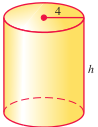
\includegraphics[scale=1]{Images/cilindro01.png} 
\end{center}
\subsection*{Pensamiento en palabras}
\item Explique como restar el polinomio $-3x^{2}+2x-4$ de $4x^{2}+6$
\item Explique como simplificar $7x-[3x-(2x-4)+2]-x$
 \end{enumerate}
 \section*{Multiplicaci\'{o}n de monomios}
 \subsection*{Conceptos}
 Conteste V o F seg\'{u}n sea el caso
 \begin{enumerate}
 \item Cuando multiplicamos dos potencias de la misma base, sumamos los exponentes
 \item $2x^{2}\cdot 3x^{3}=6x^{6}$
 \item $(-4x^{3})^{2}=-4x^{6}$
 \item $\dfrac{-8x^{6}}{2x^{2}}=-4x^{3}$
 \item $\dfrac{-14xy^{3}}{-7xy^{3}}=2$
 \end{enumerate}
 \subsection*{Problemas}
 Para los problemas siguientes, encuentre cada producto
 \begin{enumerate}
 \item $(4x^{3})(9x)$
 \item $(-2x^{2})(6x^{3})$
 \item $(-a^{2}b)(-4ab^{3})$
 \item $(x^{2}yz^{2})(-3xyz^{4})$
 \item $(5xy)(-6y^{3})$
 \item $(3a^{2}b)(9a^{2}b^{4})$
 \item $(m^{2}n)(-mn^{2})$
 \item $\left(\frac{2}{5}xy^{2}\right)\left(\frac{3}{4}x^{2}y^{4}\right)$
 \item $\left(\frac{-3}{4}ab\right)\left(\frac{1}{5}a^{2}b^{3}\right)$
 \item $\left(-\frac{1}{2}xy\right)\left(\frac{1}{3}x^{2}y^{3}\right)$
 \item $(3x)(-2x^{2})(-5x^{3})$
 \item $(-6x^{2})(3x^{3})(x^{4})$
 \item $(x^{2}y)(-3xy^{2})(x^{3}y^{3})$
 \item $(-3y^{2})(-2y^{2})(-ry^{5})$
 \item $(4ab)((-2a^{2}b)(7a)$
 \item $(-ab)(-3ab)(-6ab)$
 \item $\left(\frac{2}{3}xy\right)(-3x^{2}y)(5x^{4}y^{5})$
 \item $(12y)(-5x)\left(-\frac{5}{6}x^{4}y\right)$

Eleve cada monomio a la potencia indicada

 \item $(3xy^{2})^{3}$
 \item $(-2x^{2}y)^{5}$
 \item $(-x^{4}y^{5})^{4}$
 \item $(ab^{2}c^{3})^{6}$
 \item $(2a^{2}b^{3})^{6}$
 \item $(9xy^{4})^{2}$
 \item $(-3ab^{3})^{4}$
 \item $-(2ab^{4})$
 \item $-(xy^{2}z^{3})^{6}$
 \item $(-5a^{2}b^{2}c)^{3}$
 \item $(-xy^{4}z^{2})^{7}$
 
 Encuentre cada cociente 
 
 \item $\dfrac{9x^{4}y^{5}}{3xy^{2}}$
 \item $\dfrac{25x^{5}y^{6}}{-5x^{2}y^{4}}$
 \item $\dfrac{-54ab^{2}c^{3}}{-6abc}$
 \item $\dfrac{-18x^{2}y^{2}z^{6}}{xyz^{2}}$
 \item $\dfrac{a^{3}b^{4}c^{7}}{-abc^{5}}$
 \item $\dfrac{-72x^{2}y^{4}}{-8x^{2}y^{4}}$
 \item $\dfrac{14ab^{3}}{-14ab}$
 \item $\dfrac{-36x^{3y^{5}}}{2y^{5}}$
 
 Encuentre cada producto. Asuma que las variables representan exponentes enteros positivos.
 
 \item $(2x^{n})(3x^{2n})$
 \item $(a^{2n-1})(a^{3n+4}$
 \item $(x^{3n-2})(x^{n+2})$
 \item $(a^{5n-2}(a^{3})$
 \item $(2x^{n})(-5x^{n})$
 \item $(-3a^{2})(-4a^{n+2})$
 \item $(x^{n})(2x^{2n})(3x^{2})$
 \item $(3x^{n-1})(x^{n+1})(4x^{2-n})$
 
 Use geometría para resolver los problemas siguientes:
 
 \item Encuentre el polinomio que representa el área superficial del sólido rectangular de la figura. Encuentre también un polinomio que represente el volumen
 \begin{center}
 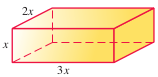
\includegraphics[scale=1]{Images/solido02.png} 
 \end{center}
 \subsection*{Pensamiento en palabras}
 \item Su amiga simplificó $2^{3}\cdot 2^{2}$ así:
 \[2^{3}\cdot 2^{2}=4^{3+2}=4^{5}=1024\]
 ¿Qu\'{e} hizo de manera incorrecta y c\'{o}mo podr\'{i}a ayudarla?
 \end{enumerate}
 \section*{Multiplicaci\'{o}n de polinomios}
 Para los siguientes puntos, multiplique usando la propiedad distributiva de la multiplicaci\'{o}n respecto de la suma. Recuerde que tambi\'{e}n puede usar los productos notables
 \begin{enumerate}
 \item $3x^{2}(6y^{2}-5x^{2}y^{4})$
 \item $-7ab^{2}(2b^{3}-3a^{2})$
 \item $9a^{3}b(2a-3b+7ab)$
 \item $-ab^{2}(5a+3b-6a^{2}b^{3})$
 \item $(t-s)(x+y)$
 \item $(a-4b)(c-d)$
 \item $(x+2)(x+10)$
 \item $(y-3)(y+9)$
 \item $(n+3)(n-12)$
 \item $(t+8)(t-8)$
 \item $(x-2)^{2}$
 \item $(x-3)(x-13)$
 \item $(x-1)((x+4)(x-6)$
 \item $(x-5)(x+5)(x-8)$
 \item $(t+13)^{2}$
 \item $(y-4)^{2}$
 \item $(6x+5)(x+3)$
 \item $(5y-2)(5y+2)$
 \item $(6x-1)(3x+2)$
 \item $(3-t)(2+4t)$
 \item $(4t+6)^{2}$
 \item $(6-3x)(6+3x)$
 \item $(5x-7)^{2}$
 \item $(4x-7)(7x+4)$
 \item $x-4y)((3x+7y)$
 \item $(9x-2y)(9x+2y)$
 \item $(t-2)(t^{2}+7t+2)$
 \item $(x+6)(2x^{2}-x-7)$
 \item $(3x+4)((2x^{2}-2x-6)$
 \item $(5x-2)(6x^{2}+2x-1)$
 \item $(x+1)^{3}$
 \item $(x-5)^{3}$
 \item $(3x+1)^{3}$
 \item $(3x-2)^{3}$
 \item $(4x-5)^{3}$
 
 Para resolver los productos indicados, asuma que las variables representan exponentes enteros positivos.
 
 \item $(x^{3a}-1)(x^{3a}+1)$
 \item $(x^{a}+4)(x^{a}-9)$
 \item $(3x^{n}+5)(4x^{n}-9)$
 \item $(x^{2a}+6)(x^{2a}-4)$
 \item $(3x^{n}-7)^{2}$
 
 Para los problemas siguientes use geometría para solucionarlos
 
 \item Explique como la figura puede usarse para demostrar geométricamente que $(x+2)(x+6)=x^{2}+8x+12$
 \begin{center}
 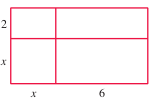
\includegraphics[scale=1]{Images/rectangulo01.png} 
 \end{center}
 \end{enumerate}
\end{multicols}


\end{document}
